\section{Procedure}
\label{sec:procedure}

\subsection{Aligning the mirrors}
\label{sec:Aligning the mirrors}
The first step is to align every optical element, where we will start with the mirrors which will
later create the cavity.

For proper alignment of the optical elements, an optical axis should be defined. We did that with a
laser on a rail, the setting of which has to be constant throughout the experiment. The laser has to
be levelled with the rail, which has been achieved with a target on the opposite end of the rail.

The mirrors can be aligned by fixing them on the rail such that the reflect the laser beam back to
the source, as it is shown in \autoref{fig:aligning}. The mirror can then be aligned with its adjustments screws.
With curved mirrors, it is important to use a proper distance to the laser source. The reflection is
the most focused when the distance is the focal distance of the mirror, though this can be to small
to get an exact aligning. We managed to get meaningful results with approx. $\SI{30}{cm}$ of
distance for the alignment.

\begin{figure}
  \centering
  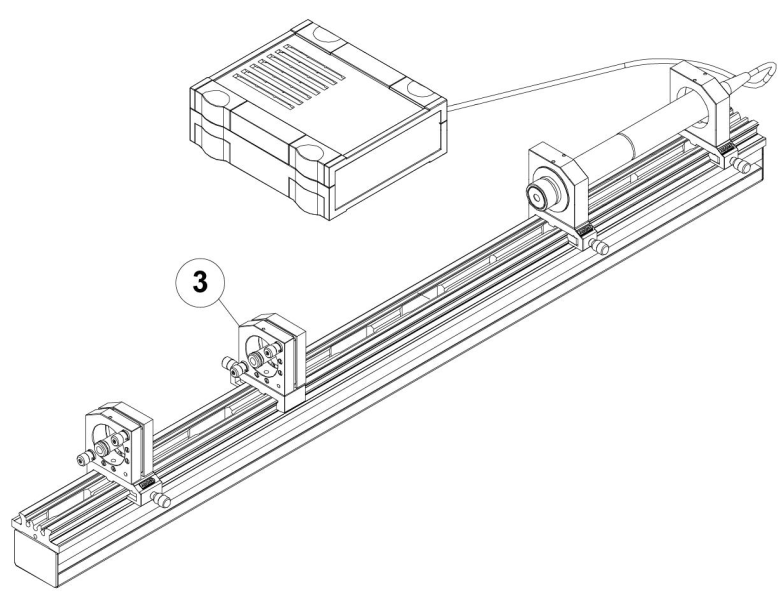
\includegraphics[width=0.45\textwidth]{media/aligning mirrors.png}
  \caption{Setup to align the mirrors. Item 3 corresponds to the mirror that can be adjusted in this
  position \cite{elas_manual}.}
  \label{fig:aligning}
\end{figure}

\subsection{Aligning the He-Ne tube}
\label{sec:Aligning the He-Ne tube}
The next step is to align the He-Ne tube, which can be done by removing the mirrors from the first
step. Than the laser and the target will be used to create a round beam shape. Here all four screws
should be used to achieve the highest range of motion.

\subsection{Creating the optical cavity}
\label{sec:Creating the optical cavity}
The last step is to position the mirrors pointing at each other with the He-Ne tube in between. Then
the reference laser can be turned off and power source of the Helium-Neon tube can be turned on.
Ideally, you get the laser oscillation right away. Practially, this is about as likely as getting an
A+ at KAIST. You can try to
shake around one mirror at a cavity length of $\SI{70}{cm}$ until you can fix it in a position where
you have a stable laser.

\begin{figure}
  \centering
  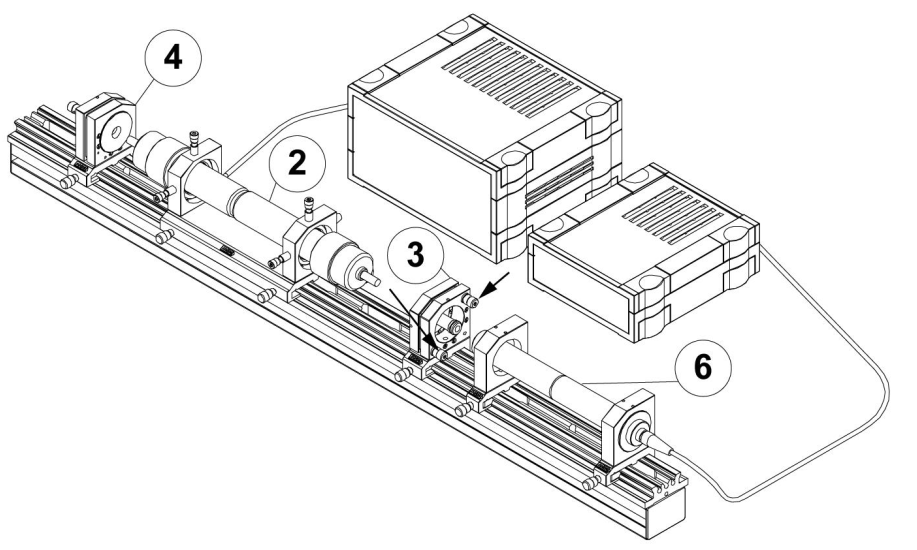
\includegraphics[width=0.45\textwidth]{media/setup.png}
  \caption{Final setup with the He-Ne tube (item 2) in the optical cavity (item 3,4). The reference laser (item 6)
  should be turned off and the He-Ne tube can be supplied with power \cite{elas_manual}.}
  \label{fig:setup}
\end{figure}
